\section{Introduction}
\label{sec:introduction}

\begin{figure*}[!t]
\floatconts{fig:thesis-overview}
{\caption{Benchmark overview. Cohorts, hourly inputs, encoder architecture, patient splits, tasks, and evaluation protocols are fixed. SSL implementations vary in their masks and auxiliary modules. Equal epochs do not imply equal compute. Baselines provide context, and TS2Vec-style illustrates extension. LOS uses mean absolute error in days.}}
{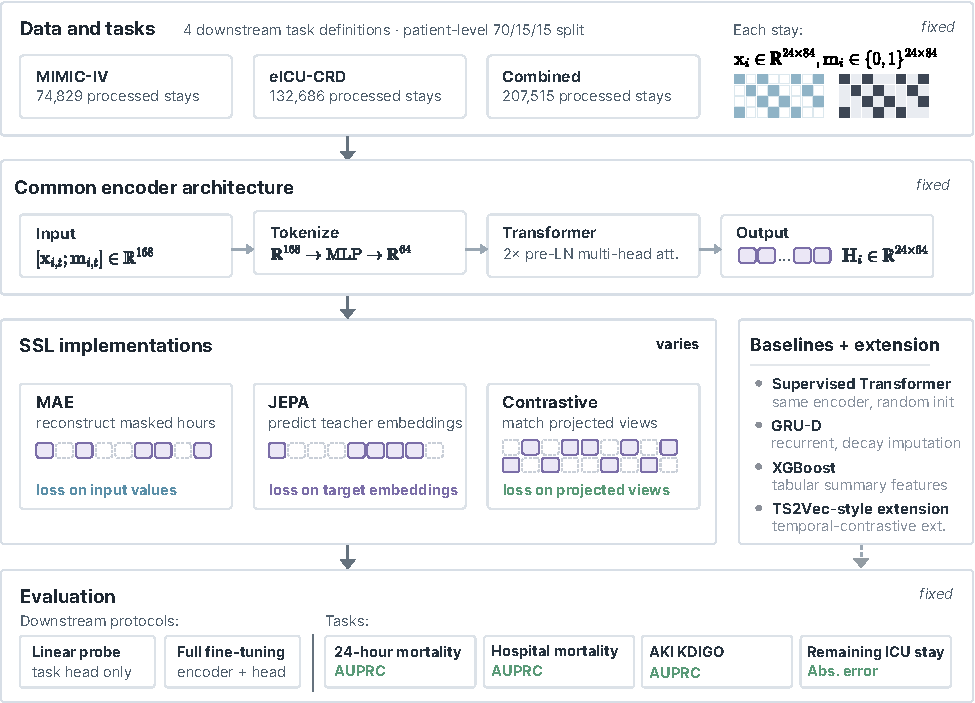
\includegraphics[width=.92\textwidth]{diagrams/fig01-benchmark-overview.pdf}}
\end{figure*}

ICU records are sparse because measurements are taken at different frequencies and often in response to a patient's evolving condition. The absence and timing of a measurement can therefore carry information about both physiology and care processes \citep{tan2023informativemissingness}. This makes ICU time series a relevant test bed for SSL. Unlabeled measurements are abundant, but the measurement process complicates the choice of learning signal.

Prior clinical SSL studies use reconstruction, forecasting, contrastive learning, or combined pretext tasks \citep{tipirneni2022strats,labach2023duett,yeche2021ncl,oufattole2024ebcl}. Their differences are hard to attribute when cohorts, representations, encoders, augmentations, and evaluation also vary. A systematic review of structured-EHR foundation models found similar heterogeneity in features, temporal representation, SSL objectives, and adaptation, with compute often underreported \citep{guo2026ehrfoundationreview}. Frozen probes test whether task information is linearly accessible. Fine-tuning tests whether a pretrained initialization remains useful after label-driven adaptation. Either alone can hide a protocol-dependent ranking.

\SLICES{} makes the evaluation contract reusable (Figure~\ref{fig:thesis-overview}). A new objective consumes the same value--mask tensors, returns a loss through a common interface, and exports the same encoder for downstream evaluation. A machine-readable specification and result validators make changes to the comparison explicit. The controlled unit is the complete implementation: masking geometry, auxiliary networks, encoder passes, and pretraining parameter counts remain objective specific.

Our contributions are:
\begin{enumerate}
  \item A benchmark framework: a fixed sparse-ICU specification, an objective/encoder-transfer interface with MAE, JEPA, and contrastive reference implementations, result validators, and a documented extension workflow. It fixes one representation, hourly values with observation masks.
  \item A first study run with the framework: 2,455 training runs across two databases and their union, with five matched seeds. GRU-D and XGBoost lead six of twelve full-label cells, fine-tuned SSL leads hospital mortality narrowly and LOS, and \MAE{} leads all frozen SSL classification comparisons. Rankings depend on the adaptation protocol, label fraction, comparator set, and probe loss.
  \item A code repository with the historical training implementation, framework code, checksummed aggregate results, and tools to regenerate results and check comparability without patient-data access.
\end{enumerate}
